  \pagebreak
  \section{Conclusiones}
    En relación con el primer experimento realizado en este trabajo
    práctico, se procede a obtener de forma analítica los valores
    de las cotas de corrección de las mediciones realizadas con
    el multímetro con respuesta al valor medio del módulo de la 
    tensión.
    
    Se sabe que los multímetros de respuesta al valor medio del
    módulo realizan una corrección mediante una cota para obtener 
    el valor eficaz de la medición. Para obtener dicha cota, se 
    hace uso de los siguientes valores representativos de una 
    \textbf{señal senoidal}

    \vspace{-5pt}
    $$ V_{RMS_{\sin}} = \dfrac{V_{\max}}{\sqrt{2}} \hspace{20pt} ; 
    \hspace{20pt} V_{|med|_{\sin}} = \dfrac{2\, V_{\max}}{\pi}~. $$

    \noindent Luego, la cota de corrección (factor de forma) se obtiene
    relacionando las expresiones anteriores
    
    \vspace{-5pt}
     $$ k = \dfrac{V_{RMS_{\sin}}}{V_{|med|_{\sin}}} 
        = \dfrac{\dfrac{V_{\max}}{\sqrt{2}}}{\dfrac{2\, V_{\max}}{\pi}}
        \hspace{20pt} \Longrightarrow \hspace{20pt} k = 1,1107~.$$

    El valor antes encontrado, es el que permite saber que el multímetro
    de respuesta al valor medio del módulo muestra en el display el 
    resultado de $ V_{lectura} = 1,1102 \cdot V_{|med|}~. $

    Teniendo en cuenta lo mencionado anteriormente, y que para una señal cuadrada
    su valor eficaz y valor medio de módulo se expresan mediante

    \vspace{-5pt}
    $$ V_{RMS_{cuad}} = V_{\max} \hspace{20pt} ; \hspace{20pt} V_{|med|_{cuad}} = V_{\max}~, $$

    \noindent entonces, la cota de corrección para la medición de 
    la señal cuadrada es

    \vspace{-5pt}
    $$ e_{cuad} [\%] = \dfrac{V_{|med|_{cuad}} - k\cdot V_{RMS_{cuad}}}{k \cdot V_{RMS_{cuad}}} \cdot 100
              = \dfrac{1,1107\, V_{\max} - V_{\max}}{V_{\max}} \cdot 100 $$
              $$  \therefore \hspace{20pt} \boxed{e_{cuad}[\%] = +11,07\%}~.
    $$

    Siguiendo la misma línea, para una señal triangular sus valor eficaz y valor
    medio de módulo se expresan mediante

    \vspace{-5pt}
$$ V_{RMS_{tri}} = \dfrac{V_{\max}}{\sqrt{3}} \hspace{20pt} ; \hspace{20pt} V_{|med|_{tri}} = \dfrac{V_{\max}}{2}~, $$

    \noindent entonces, la cota de corrección para la medición de 
    la señal triangular es

    \vspace{-5pt}
    $$ e_{tri} [\%] = \dfrac{V_{|med|_{tri}} - k\cdot V_{RMS_{tri}}}{k \cdot V_{RMS_{tri}}} \cdot 100
    = \dfrac{ 1,1107\, \dfrac{V_{\max}}{2} - \dfrac{V_{\max}}{\sqrt{3}} }{\dfrac{V_{\max}}{\sqrt{3}}} \cdot 100 $$
              $$  \therefore \hspace{20pt} \boxed{e_{tri}[\%] = -3,81\%}~.
    $$

    En la Tabla~\ref{tab:ComparacionCotas} se puede observar la comparación entre valores
    prácticos y teóricos de las mediciones realizadas con el multímetro de respuesta al 
    valor medio del módulo. Los valores presentan diferencias entre sí, en especial
    en el caso de la señal triangular. Esto se puede explicar en base a que el
    instrumento no está diseñado para medir este tipo de señales de forma correcta. 

    \begin{table}[H] \centering
      \begin{tabular}{|c|c|c|c|} \hline
        \textbf{Señal}       & \textbf{Error práctico [\%]}  & \textbf{Error teórico [\%]} & \textbf{Factor de forma} \\ \hline
        Cuadrada    & +12,16               & +11,07              &  1,000              \\ \hline
        Triangular  & -2,13                & -3,81              &  1,1547         \\ \hline
      \end{tabular}
      \caption{Tabla de comparación de cotas.}
      \label{tab:ComparacionCotas}
    \end{table}

En relación con el tercer experimento, se observó que el comportamiento del 
circuito (según la lectura del factor de potencia del dispositivo empleado), 
es de tipo inductivo, ya que al conectar el capacitor, el factor de potencia 
mejoró.

En primera instancia, se desconoce el funcionamiento interno del medidor de potencia.
Por lo que se puede suponer, que responde de manera similar a un vatímetro ideal.

Para tener un punto de partida sobre el cual analizar la razón de lo anteriormente 
expuesto, se supone las condiciones 
inciales de la siguiente manera: El TRIAC no está en región de conducción, por 
lo tanto el DIAC tampoco debería estarlo, así, ambos pueden representarse como 
un circuito abierto en el esquema de la Figura \ref{fig:CircuitoTriacDiac}. La 
segunda condición, es que el capacitor inicia totalmente descargado.

Bajo las suposiciones anteriores, el circuito resultante será el que se enseña 
en la Figura \ref{fig:ConclusionRCTriac}.

\begin{figure}[H]
  \centering
  \frame{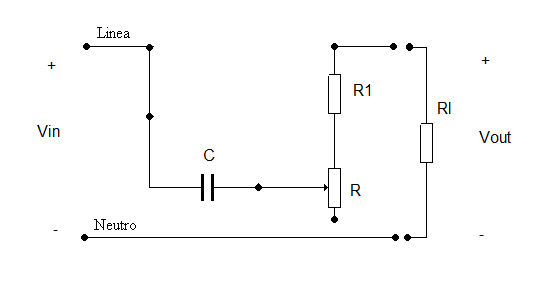
\includegraphics[width=0.8\textwidth]{Imagenes/Conclusiones/Exp3_Circuito en condicion inicial.png}}
  \caption{Situación inicial del circuito con TRIAC.}
  \label{fig:ConclusionRCTriac}
\end{figure}

Como puede observarse, se trata de un circuito adelantador de fase, cuya 
respuesta en frecuencia, puede demostrarse que se comporta como un circuito RL 
serie.

La explicación de que el dispositivo utilizado para medir el factor de potencia, 
tome al circuito como de naturaleza inductiva, se debe al adelanto de fase de la 
señal de tensión de salida, respecto de la de entrada.

Una vez que la tensión en el capacitor alcanza los 30[V] , el DIAC entra en región 
de conducción reduciendo su resistencia dinámica al mínimo, polarizando a su vez el 
TRIAC, y cerrando el ciclo de carga-descarga del capacitor. En éste punto, el sistema 
posee un comportamiento resistivo puro.

Como la condición impuesta en un principio, se mantiene 
al menos la mitad del ciclo de onda, se podría decir que tendrá comportamiento mayormente 
reactivo, de ésta manera, el dispositivo de medición determina que el circuito tiene 
características inductivas.






